% Chapter Template

\chapter{A Brief Introduction to  Coherent Raman Scattering} % Main chapter title

\label{Chapter2} % Change X to a consecutive number; for referencing this chapter elsewhere, use \ref{ChapterX}


%----------------------------------------------------------------------------------------
%	SECTION 1
%----------------------------------------------------------------------------------------
\section{A Brief History of Nonlinear Microscopy}
Since the invention of the microscope, the role of optics in understanding biology and medicine has been difficult to overstate. During the middle and late twentieth century, many new techniques such as phase-contrast, differential interference contrast, and darkfield contrast were developed that expanded the role of microscopy and opened many new aspects of the microscopic world to investigation. The first theoretical prediction of multiphoton phenomena occurred in 1931, and the first demonstration was not until after the invention of the laser enabled access to high energy density, coherent sources of light.~\cite{Mayer31,PhysRevLett.7.229} Afterwards, nonlinear microscopy techniques, e.g. second harmonic generation (SHG), two-photon excited fluorescence (TPEF), third-harmonic generation (THG), were   developed at the turn of the twenty-first century, evolving from experimental work done in spectroscopy and laser development over the preceding decades. \cite{HELLWARTH1974318,Fine:71,Freund:86,Denk73}

During this same period, the development of Raman spectroscopy and its use as a microscopic tool accompanied the invention of the  various refractive contrast methods, harmonic generation spectroscopies, and many fluorescence techniques.~\cite{RAMAN:1928aa, doi:10.1002/jrs.1486}  Raman spectroscopy provides a means of studying the chemical constituents of a sample. The information available in a Raman experiment includes chemical subgroups, their relative concentration to one another, bond strength and dynamics, and molecular symmetry.  Raman spectroscopy is often said to give a \textit{fingerprint} from which to identify molecules.~\cite{doi:10.1080/05704928.2014.923902}  Raman has proven to be a powerful tool in many areas including gas phase, condensed matter, and more recently biology.  However, it it not without its weaknesses.  Raman measurements are notoriously slow, and it is often difficult to extract the weak Raman scattering signal from a large fluorescent background.  

The origin of the Raman effect is inherently found within quantum mechanics, and it is within that framework that several alternatives to it can be found. Much as G{\"o}ppert-Mayer predicted multiphoton absorption and emission to act as counterpart to linear absorption and fluorescence, so to were a set of phenomena analogous to Raman scattering discovered and characterized.~\cite{PhysRevLett.9.455, PhysRevLett.11.160, PhysRev.130.1850} Of particular note, are Coherent Anti-Stokes Raman Scattering (CARS) and Stimulated Raman Scattering (SRS). Collectively, they fall into the classification of Coherent Raman Scattering (CRS) techniques.  These two phenomenon provide information that is based on to the linear Raman spectra, but rely on different experimental parameters.  Depending on the information to be obtained, these experiments can often lead to quicker examination of a sample. 

Much as application of harmonic generation and two-photon fluorescence into the biologist's microscope lagged behind their spectroscopic applications, the first application of CRS technology towards a biological problem did not occur until 1999.~\cite{PhysRevLett.82.4142} Following this successful demonstration of a CARS microscope, the field of CRS imaging bloomed with many studies being published over the next decade.~\cite{Potma:2001aa, Cheng:2004aa, Evans:2008aa} SRS as a phenomenon had been demonstrated almost as soon as the laser had been invented. It was quickly realized that it could be harnessed as a technique to shift the frequency of a laser line. This field of work has seen significant progress, and it has been applied in the field of optics communication and in Raman-based fiber lasers.  

However, its application as a spectroscopic and/or microscopic tool significantly lagged. The first demonstration of an SRS microscope occurred in 2007, and was quickly followed the next year with an application to biological systems.~\cite{Ploetz2007, Freudiger1857}  Since these first demonstrations, the applicability of SRS microscopy to address fundamental and applied biological questions has been clearly demonstrated with many contributions from several different research groups and a number of review articles.~\cite{Prince:2017aa, C5CS00693G, FU201724}  Recently several groups, including ours, have pioneered the application of isotopic and small functional group tags in SRS.~\cite{C8AN00910D, Hou2503,Wei:2016aa, Alfonso-Garcia2015}

\section{Overview of the Theory of Coherent Raman Scattering}

An extended version of this section can be found in:

R. C. Prince, R. R. Frontiera, and E. O. Potma, "Stimulated Raman Scattering: From Bulk to Nano", \textit{Chemical Reviews} {\bf117}(7), 2017, 5070--5094

SRS is one of a group of third-order nonlinear interactions that arise from the interaction of high intensity light fields with matter.  By taking the perspective of the light fields, it is easy to see the connection to linear Raman scattering.  From there, it is possible to examine the interaction from a semi-classical point of view; wherein the light is viewed in the classical field picture, but the material properties are described quantum mechanically.

\begin{figure}[h]
    \centering
    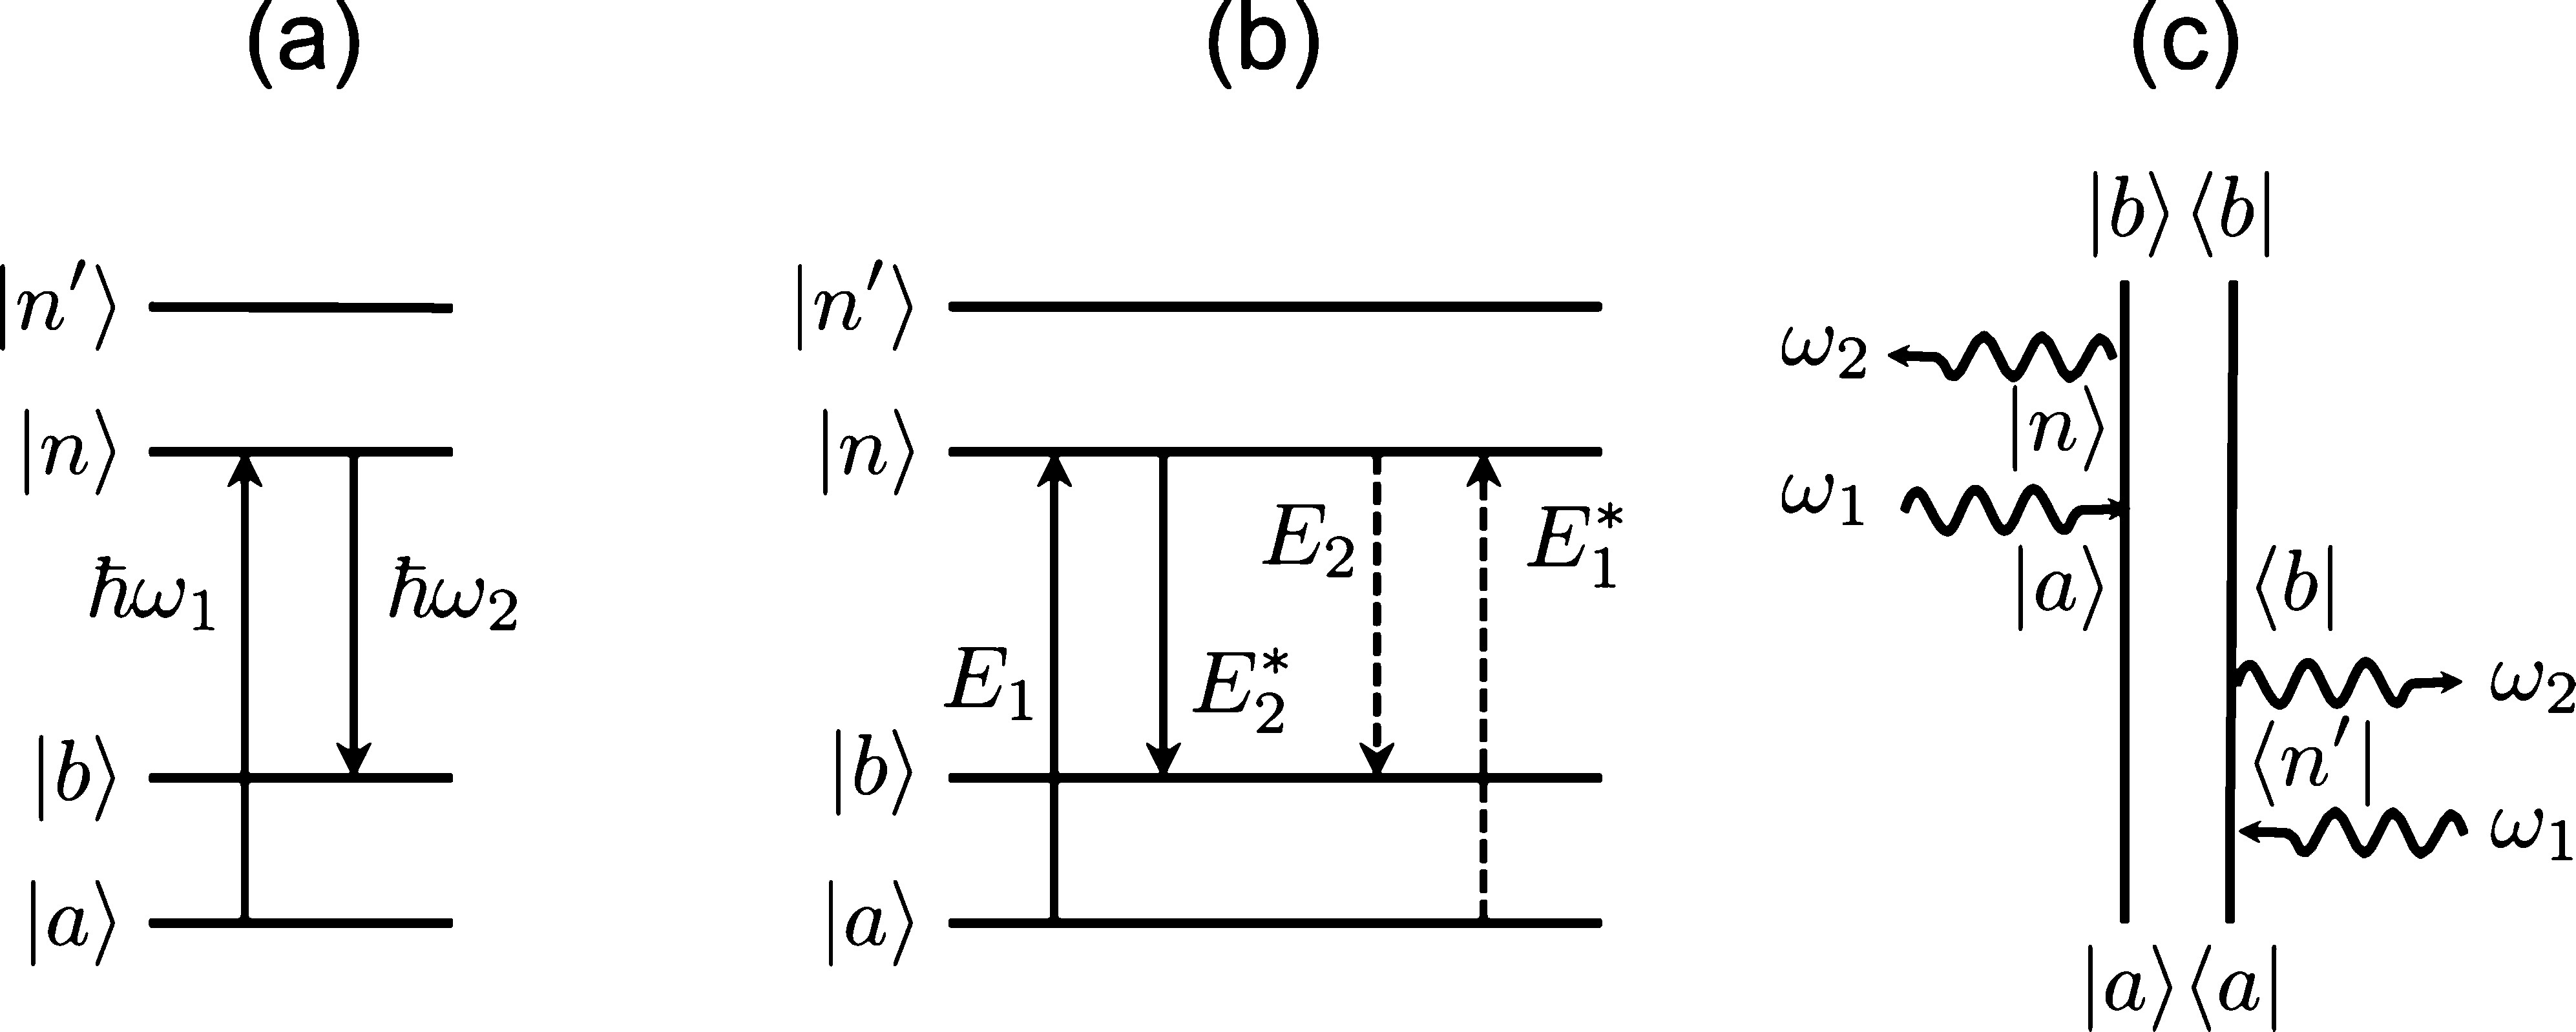
\includegraphics[width=.9\textwidth]{Figures/jablonski}
    
    \caption{Schematic of the SRS light–matter interaction. (a) Jablonski diagram in the intensity representation showing the absorption of an $\omega_1$ photon and the emission of a $\omega_2$ photon. In all cases, the states $\ket{n}$ and $\ket{n'}$ are dummy states that can be representative of the mediating virtual state. (b) Field Representation diagram Fields $E_1$ and $E_2$ interact with the quantum mechanical states of the material. Note that the arrows are not time-ordered. (c) Double sided Feynman diagram of one of the SRS pathways. \label{fig1}}
    
\end{figure}

In the linear Raman process, light incident on a material scatters inelastically. The light can either excite vibrational motion in the material in which energy is loss from the field causing the light to shift to longer wavelengths, a process known as Stokes scattering, or the light can absorb energy from existing vibrations in the material, a process known as anti-Stokes scattering.  In the situation of Stokes scattering, is is fairly easy to understand that for a given incident light field with frequency $\omega_1$ the generation of vibrational motion in the sample at a resonant frequency $\omega_R$ will result in the annihilation of and $\omega_1$ photon and generation of a red-shifted photon at frequency $\omega_2$. The difference in energy of the incident and scattered photon $\hbar(\omega_1-\omega_2)$ is equal to the energy of the vibrational mode $\hbar\omega_R$.  This is shown diagrammatically in \ref{fig1} in which the incident photon at $\omega_1$ is absorbed and a Stokes photon at $\omega_2$ is emitted.  This process happens simultaneously and is said to be mediated through the virtual state, $\ket{n}$.  The mediation of the virtual state is what allows this process to occur even though there is often no electronic eigenstate that coincides with the energy of the incident light.

Raman in an inherently weak process. Of the light incident on a given sample nearly all of it is scattered elastically through Rayleigh scattering.  In Raman, the scattered photon must be provided by the vacuum field.  In terms of the occupation number of the photon modes, the Raman process changes the occupation number of the $\omega_1$ mode originally $n_1>>1$ to $n_1-1$, and the occupation of the $\omega_2$ mode, originally $n_2=0$, to $n_2+1$.  The Jablonski diagram for stimulated Raman scattering is the same as for linear Raman, and is shown in its intensity form in \ref{fig1} panel a.  However, in SRS the $\omega_2$ field is populated by a large number of photons, $n_2>>1$.  In SRS, the rate of photon generation in the $\omega_2$ channel, $W_{stim}$, is proportional to both the $n_1$ and $n_2$ occupation numbers, i.e. $n_1(n_2+1)$~\cite{Hellwarth1963}. On the other hand, for spontaneous Raman scattering the rate of emission, $W_{spon}$, is proportional to $n_1$, because $n_2=0$. The effect of the stimulating field is thus to increase the rate of $\omega_2$ emission~\cite{Crampton2016}:
\begin{equation}
\frac{W_{stim}}{W_{spon}}\propto n_2 + 1\label{eq:stimspon}
\end{equation}
As shown above, the high population number of the $\omega_2$ field greatly increases the rate of conversion of photons from the $\omega_1$ beam to the $\omega_2$.  In fact, the stimulation effect allows for information about the Raman transition to be retrieved at at a rate many orders of magnitude faster than in linear Raman scattering. This process has been dubbed stimulated Raman scattering as it is analogous to the stimulated fluorescence emission most notably responsible for the coherent production of lights in lasers. It has been demonstrated that the typical increase in signal acquisition rate from a microscopic probing volume typically exceeds $10^5$ for SRS over spontaneous Raman. In this limit, SRS offers clear benefits. For instance, if a spontaneous Raman measurement of a particular vibrational mode takes 100 ms, SRS can provide the same information with comparable S/N in only 1 $\mu$s.  

With the annihilation of an $\omega_1$ photon and emission of an $\omega_2$ photon there is a simultaneous excitation of a vibrational mode in the material. While the intensity diagram is useful for understanding the process, it does not give an entirely clear picture.  Panel b in \ref{fig1} underscores the nonlinear nature of the SRS process by showing the scattering event in terms of the electric fields involved (as opposed to the photon energies).  From this it is clear that SRS is a four-wave mixing process. By keeping track of these fields and their interactions in a time-ordered fashion, it is possible to understand the evolution of quantum coherence within the material.  

While a full quantum dynamical treatment is beyond the scope of this work, it is useful to describe the process represented by panel c in \ref{fig1}. The system starts out in the ground state, indicated by the $\left|a\right>\left<a\right|$ population at the bottom of the diagram. The first light-matter interaction is with the field of frequency $\omega_1$, which changes the bra from $\left<a\right|$ to $\left<n'\right|$. The states indicated by $n$ and $n'$ can be either real or virtual states. For ground state SRS, these electronic states are virtual states and the $n,n'$ labels are dummy indices. The second field interaction on the bra side generates the coherence $\left|a\right>\left<b\right|$. This is the Raman coherence in the material which, in the absence of fields, evolves according to the unperturbed Hamiltonian $\hat{H}_0$. The density matrix $\rho_{ab}$ is said to propagate during this period, tracking the time-dependent material response to the light-induced superposition of the ground state and the vibrationally excited states. The density matrix is then interacting with fields $\omega_1$ and $\omega_2$ on the ket side, generating the population $\left|b\right>\left<b\right|$.

When the $\omega_1$ and $\omega_2$ fields are coincident in time, the SRS process is instantaneous on the timescale of the vibrational coherence. This implies that the emitted field maintains a definite phase relation with the incident light fields. As a consequence, the SRS signal is coherent. Since this is true for every scatterer in the excitation volume, the combined radiation from the scatterers exhibits coherence as well. Spatial coherence within the excitation volume results in the coherent propagation of the signal in the so-called phase matched direction, i.e. the direction in which the radiating scatterers produce fields that are in-phase. To summarize from this diagram, the SRS interaction has moved population from the ground state to the first vibrationally excited state, and in doing so produced a coherent signal that will propagates into the far-field along the phase-matched direction. 

In order to understand the nature of the vibrationally excited states probed by both spontaneous Raman and SRS, it is necessary to examine the coupling between atoms in molecular bonds. The frequency of the incident radiation is typically in the visible to near-infrared range ($\Tilde{10^3}$ THz), whereas the frequencies of the nuclear vibrational motions in molecules are of much lower frequencies (1–100 THz). Therefore, the nuclei cannot follow the incident fields adiabatically. Instead, the molecules couple to the fields through their electrons, which can follow the rapid oscillations of the driving fields. In case there is coupling between the electron motions and the nuclear modes, the resultant electron oscillation contains information about the nuclear vibrations as well. Raman processes thus probe nuclear motions in the molecule indirectly through the motion of electrons. In SRS, the process reports on these motions through the transfer of photon energy from the $\omega_1$, or pump, beam to the $\omega_2$, or Stokes, beam. This transfer of photon energy creates two different opportunity to measure the response of the material optically in the far-field.  

\begin{eqnarray}
S_{SRG}(\omega_2)&\propto&\left|A_1\right|^2\left|A_2\right|^2Im\left\{\chi_{NL}(\Omega)\right\}\label{eq:srg}\\
S_{SRL}(\omega_1)&\propto&-\left|A_1\right|^2\left|A_2\right|^2 Im\left\{\chi_{NL}(\Omega)\right\}\label{eq:srl}
\end{eqnarray}  

Equations \ref{eq:srg} and \ref{eq:srl} show that the signal at the detector can be measured as either a gain in the Stokes beam or loss in the pump.  In both cases, the signal is linearly proportional to the intensity of the two beams as intensity is directly proportional to the square of the amplitudes of each field.  Additionally, these equations include the nonlinear response of the material through inclusion of the $\chi_{NL} (\Omega)$ term.  This is the the nonlinear susceptibility of the material and includes the fundamental selection rule for the Raman phenomenon that relates the coupling of the electron motions to the nuclear modes of the molecule.   This is shown explicitly in \ref{eq:chi} by the derivative term.  A full mathematical treatment can be found in \textit{Coherent Raman Scattering Microscopy, 2013, CRC Press}.\cite{Potma:2013aa}


\begin{equation}
\chi_{NL}(\Omega)=\frac{N}{6m\epsilon_0}\left(\frac{\partial\alpha}{\partial Q}\right)^2_0 \frac{1}{\omega^2_\nu-\Omega^2-2i\Omega\gamma}\label{eq:chi}
\end{equation}


From the theory, it is evident that SRS is capable of probing the same vibrational modes as spontaneous Raman, and in fact can do so at much higher rates.  The theory also shows that the optical effect induced in this way is capable of carrying information into the far field. At the far field, it is possible to measure the transfer of energy from one field to the other, and from this spectroscopic information can be obtained.  Knowing the spectroscopy then leads to an ability to produce contrast in an optical microscope.  

\section{The Narrowband SRS Microscope}
\begin{figure}[h]
    \centering
    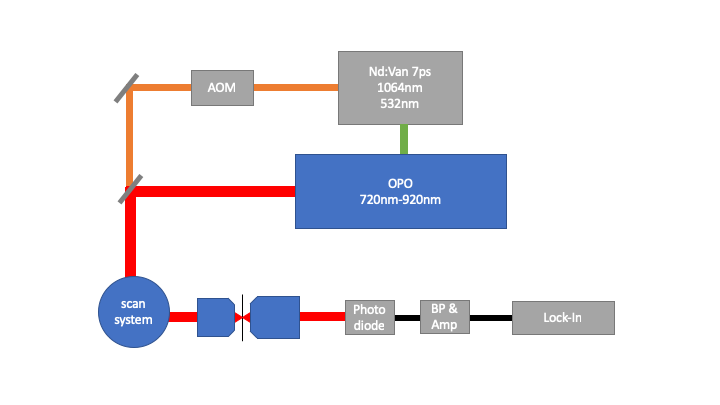
\includegraphics[width=.9\textwidth]{Figures/Slide1.png}
    \caption{A Schematic Representation of the Narrowband SRS Microscope \label{scope}}
\end{figure}
The implementation of a high-resolution SRS microscope in our case is similar to other laser-scanning multi-photon systems.  A basic schematic is shown in \ref{scope}.  While it is possible to generate the SRS signal with several different excitation schemes, each has its own advantages or disadvantages.  Previous work has shown, that high spectral resolution is achieved with the use of picosecond pulses as both the Stokes and pump beams.  This allows for resolution on the order of $\sim10cm^{-1}$.  . Additionally by tuning to match specific Raman resonances such that $\Omega_R$ = $\hbar\omega_{pump}-\omega_{stokes}$ it is possible to build high resolution spectra of entire images. This capability for fast acquisition of a large spectral dataset at every pixel in an image allows for direct comparison to spontaneous Raman spectra, and the usefulness of this technique will be discussed later in this work. It is apparent from the description of the SRS process that the use of colinear picosecond pulses necessitates the use of a modulation scheme in order to resolve the rather minuscule SRL or SRG signal that propagates with the incident beams in the forward direction.

To discriminate the SRS signal from the laser light, the use of high-frequency modulation ($\sim10\;MHz)$ is required.  Modulation in this frequency range allows the SRS system to approach the shot noise limit as most laser noise occurs at lower frequencies.  In the case of SRL detection, an amplitude modulation is applied to the Stokes beam through the use of an acousto-optic modulator.  During the interaction with the sample, this modulation is transferred from the Stokes to the pump.  Demodulation of the signal after detection can be accomplished through the use of high-speed lock-in amplifiers. A diagram of the modulation scheme is shown in \ref{fig:mod}.

\begin{figure}[h]
    \centering
    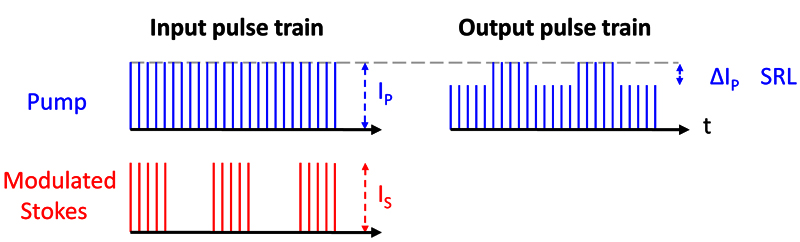
\includegraphics[width=.8\linewidth]{Figures/SRSmodualtionScheme.jpg}
    \caption{Modulation in SRS:  A high frequency modulation is applied to the stokes beam by an AOM.  This modulation is then transferred onto the pump during the SRS process.  Adapted from \cite{Freudiger1857}}
    \label{fig:mod}
\end{figure}

In all instances described in the remaining sections of this work, SRL is measured using a combination of a fixed stokes beam at 1064nm generated by a 76-MHz mode-locked Nd:Vanadate laser (Picotrain, High-Q, Hohenems, Austria) delivering 7 picosecond width pulses and a variable pump beam generated through an optical parametric oscillator (OPO; Levante Emerald, APE, Berlin Germany) pumped by the second harmonic of the laser at 532nm. For SRL, the stokes beam was modulated at 10MHz using an acousto-optic modulator (AOM, Crystal Technology, Palo Alto, California). After modulation, the two beams are combined both spatially and temporally and directed into a laser scanning inverted microscope (Fluoview 300 \& IX71, Olympus, Center Valley, Pennsylvania). The beams are raster scanned through a high NA objective onto the sample. The SRS signal is collected in the forward direction by a high NA condenser.  This is necessary as mismatch between the NA of the objective and the NA of the condenser can lead to spurious signal in the form of cross-phase modulation and thermal lensing. The pump beam is passed trough a dichroic filter and is incident onto a silicon photodiode.  After detection, unwanted frequency components were initially filtered by an inline 10MHz bandpass filter (BBP-10.7+, Mini-Circuits, Brooklyn, New York). The remaining signal is passed through an analog voltage amplifier (HVA-10M-60B, Fempto, Berlin) and connected to the input terminal of a lock-in amplifier (HF2LI, Zurich Instruments, Zurich, Switzerland). The use of the high0speed lock-in amplifier allows for demodulation of the relatively weak Raman loss signal from the much stronger pump signal detected at the photodiode. The time constant of the lock in was set to match the pixel dwell time for optimal S/N. The SRS signal is collected on an output channel of the lock-in by the synced Fluoview system to form the intensity image. 

\begin{figure}[h]
    \centering
    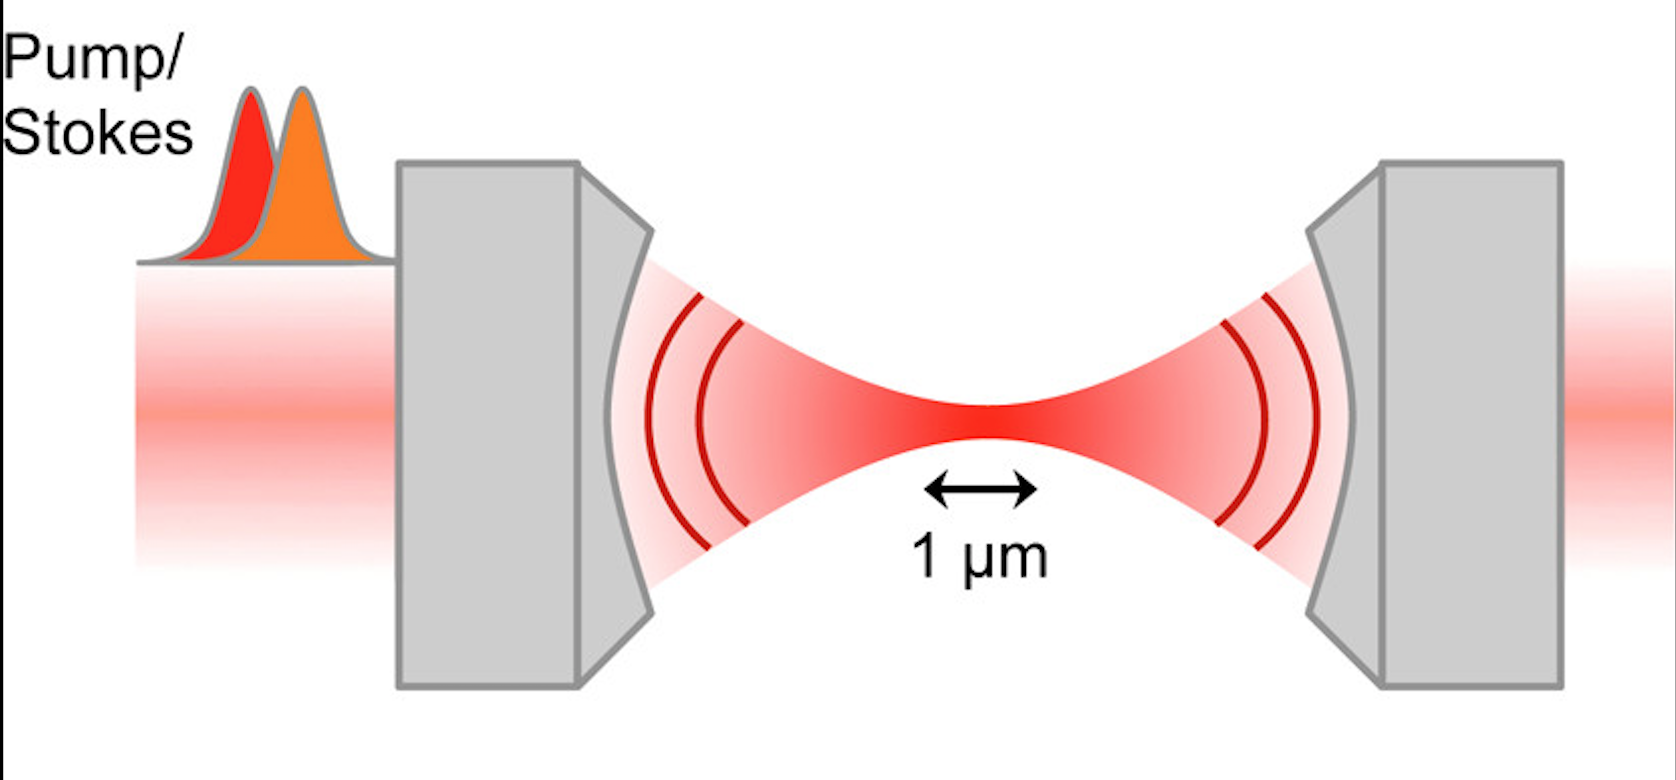
\includegraphics[width=.7\linewidth]{Figures/focal.png}
    \caption{Microscope configuration where the incident beams are focused in collinear fashion with a high numerical aperture lens to a diffraction-limited interaction volume$\Tilde{1\mu m^3}$}
    \label{fig:focal}
\end{figure}

When working with microscopic probing volumes it is necessary to understand and take into consideration several effects of wave optics. A graphical representation of collinear excitation is shown in \ref{fig:focal}. Under high NA conditions, the interaction volume has a length of only $\sim{1\mu m}$, which is on the order of an optical wavelength. In this limit, the phase-matching condition $\Delta\Phi<\pi$ can be fulfilled even if $\Delta k \neq 0 $. For the forward propagating direction in SRS, we have $\Delta k = 0$, so the signal is phase-matched in this direction regardless. The use of high numerical aperture lenses can reduce the sampling volume to about a fL. Although such a volume is much smaller by many orders of magnitude as compared to volumes encountered under macroscopic focusing conditions, it is still far removed from the molecular scale. For example, 1 fL of water contains no less than $10^10$ water molecules.  Within this regime, it is possible to generate high-quality images by tuning to specific Raman resonances.  In this way, chemical selectivity is achieved and only those areas containing a high concentration of emitters will produce signal.  Additionally, as SRS probes the imaginary part of the susceptibility there is no nonresonant background to reduce contrast.

\section{Information from an SRS Experiment}

As was alluded to in the sections above, it is possible to gain a wealth of information from the SRS experiment on microscopic samples. A brief description is provided here, and specific examples will be shown and discussed in the sections on current work and the research plan.

\begin{figure}[h]
    \centering
    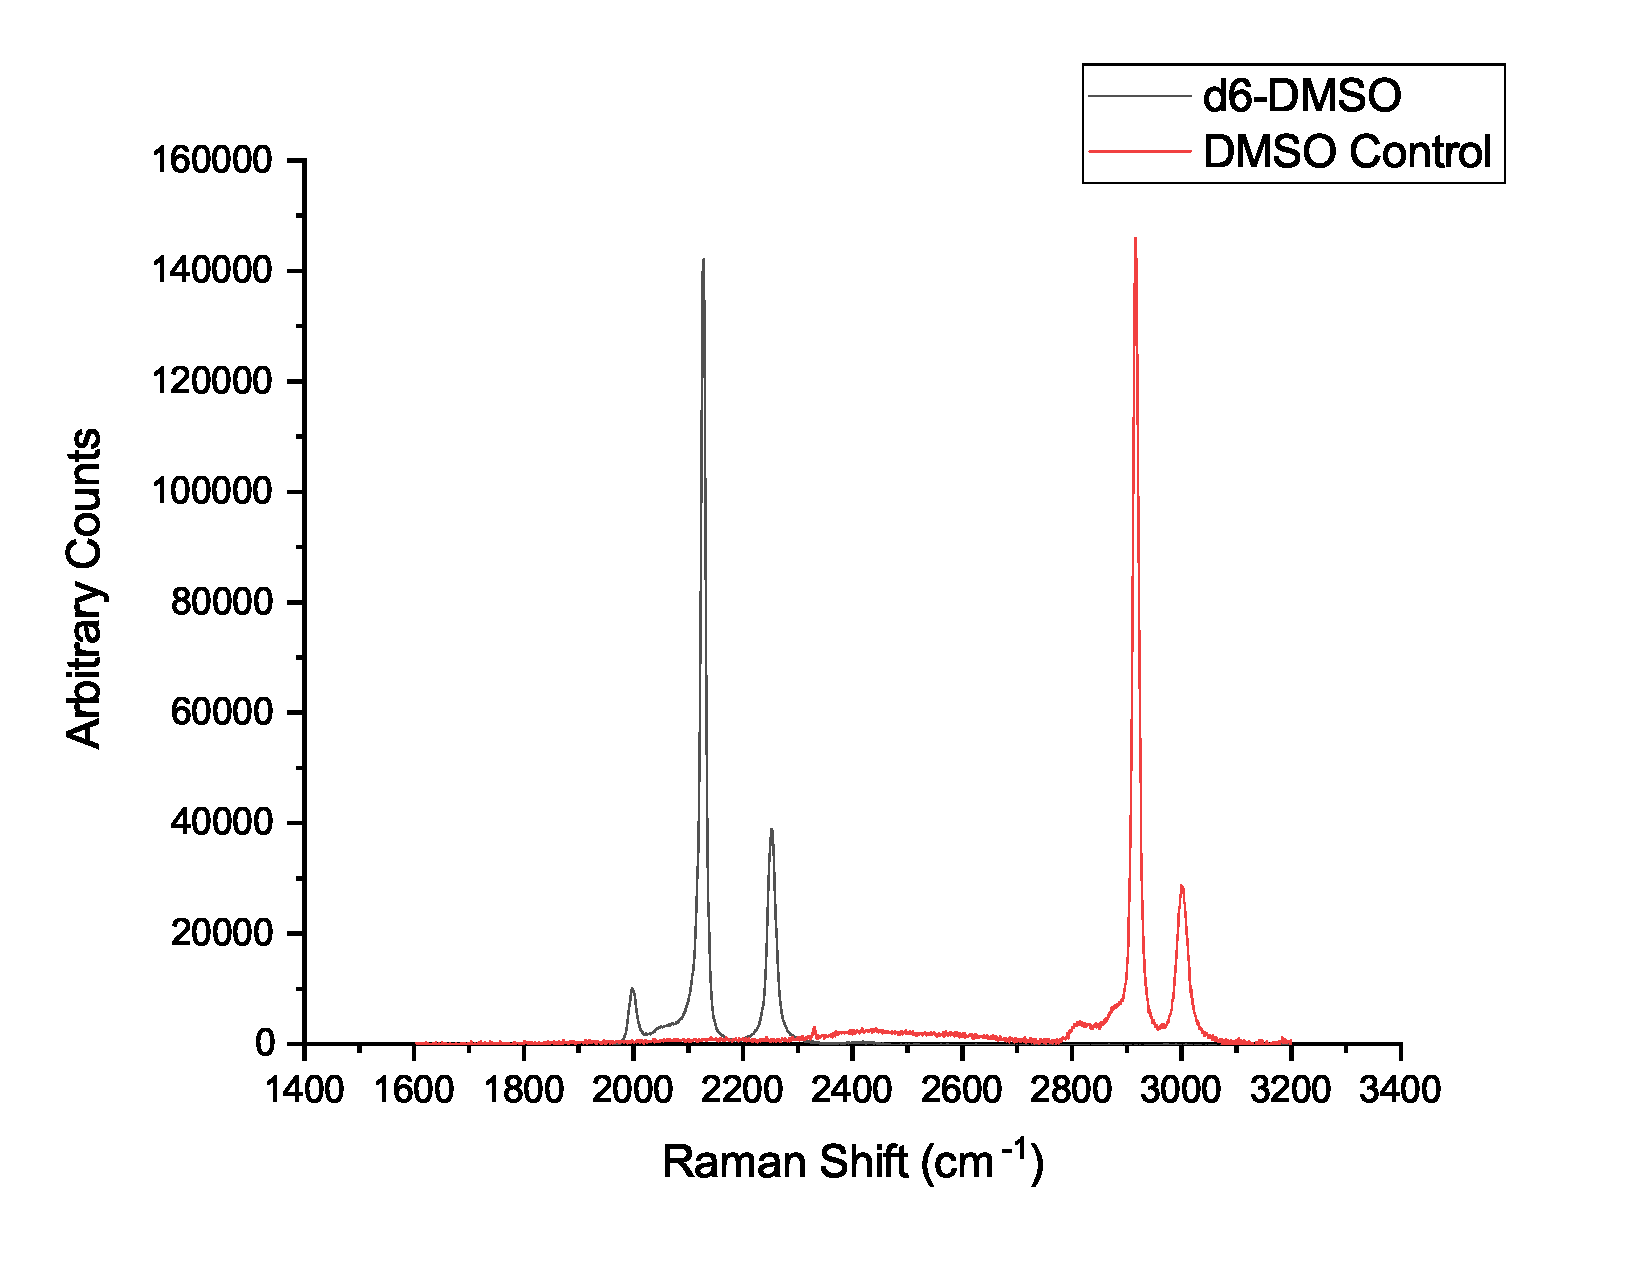
\includegraphics[width=.7\linewidth]{Figures/dmso.eps}
    \caption{Raman Spectra of normal DMSO and deuterated DMSO.}
    \label{fig:spec}
\end{figure}

As Raman scattering spectroscopy probes the various vibrations of molecular bonds it is possible to retrieve a large amount of information from the Raman spectrum. An example of the spectra of DMSO and it's deuterated version are provided in Figure \ref{fig:spec}.~\cite{C6RA25879D} In these spectra, functional group vibrational modes are recognizable in the form of the CH modes centered around 2900$cm^-1$. The comparison of these two spectra show how a slight adjustment in the reduced mass of the oscillator, in this case substituting deuterium for hydrogen, makes a large difference in the position of the Raman peaks.  Detailed analysis of hyperspectral images in SRS, such as that provided with principle component analysis, can utilize this information to produce chemical contrast for images by varying the wavelength of the pump beam over a series of images. In fact, as shown in \cite{Alfonso-Garcia2015}, a range much smaller than that shown in \ref{fig:spec} can provide enough information to sort out differences in compounds such as protein and lipid. Additionally, rapid imaging at one band is available on the order of one frame per second. This creates the ability of SRS to generate images mapping the location of select functional groups in cells and tissues. 

\begin{figure}[ht]
    \centering
    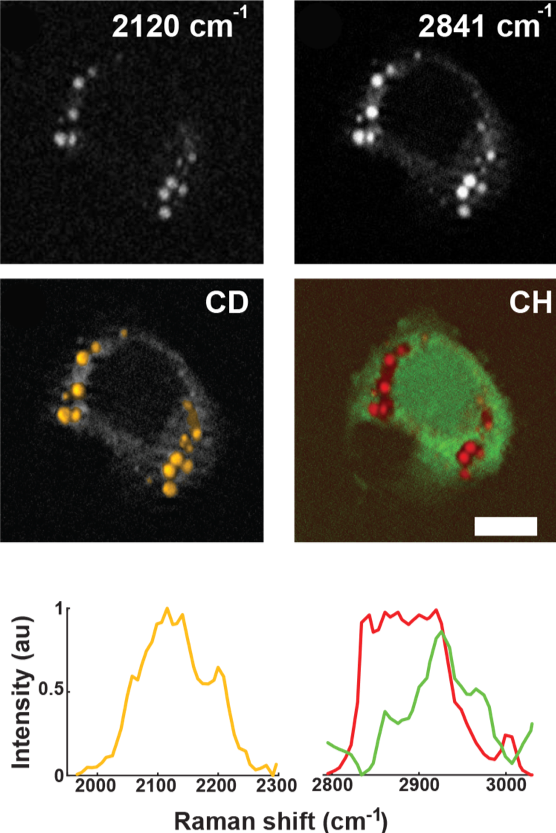
\includegraphics[width=0.5\linewidth]{Figures/dchol.png}
    \caption{SRS imaging at  2120 $cm^-1$ corresponding to CD2 stretches and 2841 $cm^-1$ corresponding to CH2 symmetric stretches. The result of hyperspectral SRS imaging and multivariate analysis is depicted in yellow for D38-cholesterol in the CD region , overlaid on the maximum intensity projection of the CH spectral scan in gray scale, and in red for lipid and green for protein in the CH region.}
    \label{fig:dchol}
\end{figure}

As will be discussed in the section on current work, the addition of small molecule or isotopic tags allows for high chemical contrast not otherwise present in the cell.  An example of this is provided in \ref{fig:dchol} from a previous project in our lab.\cite{Alfonso-Garcia2015}  This image shows how SRS imaging over only a narrow range of wavelengths allows for the colocalization of cholesterol in lipid droplets after esterification. Additionally, as the image shows, with high enough spectral resolution it is possible to separate protein and lipid just based on their signatures in the CH spectral region.








 




